\documentclass[mscthesis]{usiinfthesis}
\usepackage{lipsum}
\usepackage{xcolor}
\usepackage{float}
\usepackage{cleveref}
\usepackage{makecell}
\usepackage{colortbl}
\usepackage{pdflscape}

\usepackage{listings}

\lstdefinelanguage{algebra}
{morekeywords={import,sort,constructors,observers,transformers,axioms,if,
else,end},
sensitive=false,
morecomment=[l]{//s},
}



\title{Design and implementation of a firewall system for working in unsafe environments} %compulsory
\mastermajor{Financial Technology and Computing}%optional
\specialization{main track}
%\subtitle{Subtitle: Reinventing the World} %optional 
\author{Bin Yong} %compulsory
\begin{committee}
\advisor{Prof.}{Student's}{Advisor} %compulsory
\coadvisor{Prof.}{Student's}{Co-Advisor}{} %optional
\end{committee}
\Day{Yesterday} %compulsory
\Month{September} %compulsory
\Year{2023} %compulsory, put only the year
\place{Lugano} %compulsory

%\dedication{To my beloved} %optional
%\openepigraph{Someone said \dots}{Someone} %optional

%\makeindex %optional, also comment out \theindex at the end

\begin{document}

\definecolor{tablegray}{gray}{0.85}

\maketitle %generates the titlepage, this is FIXED

\frontmatter %generates the frontmatter, this is FIXED

\begin{abstract}
  \paragraph{}
  Design and implementation of a firewall system based on Raspberry Pi. The firewall monitors network activities and encrypts some plaintext traffic. It helps device owners take back control of their own devices. It is designed for someone who needs to work in unsafe environments. The system sacrificed some compatibility to pursue better security but still achieved a balance between security and convenience. A sensitive target, like an investigative journalist, could be a potential user of this device.

\end{abstract}

\begin{acknowledgements}
  \paragraph{}
  This document is a draft version of a working thesis of Bin Yong. It is licensed under Creative Commons BY-NC-ND 4.0.
\end{acknowledgements}

\tableofcontents
\listoffigures %optional
\listoftables %optional

\mainmatter

\chapter{Introduction}
\paragraph{}
With the development of surveillance and management tools, people are losing control of their own devices. Here are some facts that the general public may underestimated the impacts of their combinations:

\begin{table}[H]
  \begin{enumerate}
    \item Any device with a microphone (sometimes a speaker may do the same) can 'hear' sounds people are making around.
    \item Any device with a camera can 'see' what is happening around.
    \item Any device connected to internet can upload what they know and receive commands from remote.
    \item Any device may have been hacked and functioning as not what they were designed.
    \item Some devices are designed with surveillance functionality.
  \end{enumerate}
  \caption{Some facts}
  \label{lst:facts}
\end{table}
Based on the facts above, some devices are naturally born with surveillance abilities. For example, smartphones and smart speakers are both able to hear voices and communicate with the internet. Most people do not have the skills to investigate and monitor what they actually uploaded to a remote server. To make them able to respond to "Hi, Siri." or "Hey, Alexa.", those devices have to process every sound they receive when they are quiet. Some are even worse: Intel Management Engine (Intel ME) or Intel Converged Security and Management Engine (Intel CSME) and Intel Active Management Technology (Intel AMT) for example. It's obvious that they are made for management, a function that is unnecessary to most individual owners. According to their official documents. "its power stats are independent" means that simply powering off the computer could not stop this management. "up before the main operating system" means that most users could not even notice it and could do nothing about it, and if something goes wrong, people cannot fix it by simply reinstalling operating system. It can access "LAN/Wireless LAN", check \cref{lst:facts}. "present on most Intel platforms, including client consumer and commercial systems, workstations, servers, and IoT (Internet of Things) products." means there is almost no escape in their ecosystem. The details of its documents also show the capability of running remote commands (Serial Over Local-Area Network), the capability of accessing local storage "Universial Serial Bus Redirect", "Keyboard, Video and Mouse" remote control over network.
\paragraph{}
So many things are out of the control of the owners of the devices. People need something to restrict the management and to show what is happening to the network. The goal of this work is to help with that. It aims to increase the chance of survival of the user from hacking, eavesdropping, digital fingerprinting, and unwanted managements. It uses a screen to display selected real-time internet activities. The system limits network activities and applies encryption standards.
\paragraph{}
Using hardware firewalls has several advantages over software firewalls. Firstly, a hardware firewall runs completely independent to high-risk user devices, where unsafety thrives: CPU with possible hidden instruments, firmware with possible infections, motherboards with doubtable proprietary management technologies, and applications with possible surveillance or unpublished vulnerabilities. Second, it brings convenience to the user: the configuration of this portable device restricts everything behind it, so people do not need to do the time-consuming configuration work on different software and operating systems repeatedly. Third, it brings possibilities: Untrusting a built-in root certificate on mobile devices is hard and the methods with root or jailbreak involved may void the warranty. With the help of a firewall, managing certificates is no longer a problem.
\paragraph{}
This firewall system evaluated threats faced on different aspects by a network device and provided some unique solutions.

\chapter{Hardware}
\section{Design}
\paragraph{}
Hood should work as a USB ethernet device by default, so people do not need to connect many cables. See \cref{fig:hardware-deployment-view}. With proper configurations, the device itself can also work as a wireless access point or a wireless USB ethernet device. The cost of the hardware should be lower than the average price of a commercial hardware firewall.
\begin{figure}[H]
  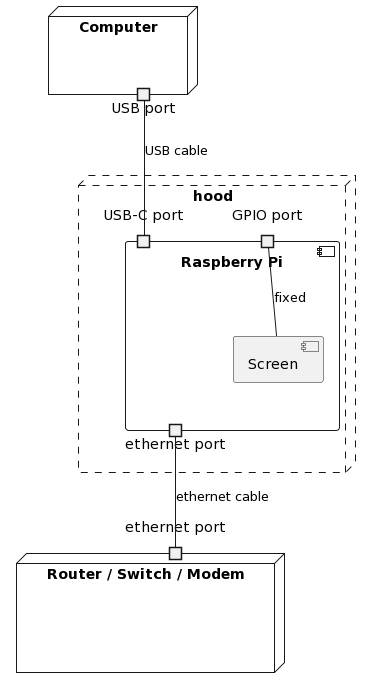
\includegraphics[scale=1]{graphics/puml/hardware-deployment-view.png}
  \caption{Default hardware deployment view}
  \label{fig:hardware-deployment-view}
\end{figure}

\section{Implementation}
\subsection{USB device}
\paragraph{}
To make computers recognize the firewall as a USB device, the support from both the development board and the operating systems (OS) are required.
\paragraph{}
For hardware, Raspberry Pi 4 is the first model in Raspberry Pi family that both supports USB device mode and contains a ethernet port. Raspberry Pi 5 can do the same but it is more expensive.
\paragraph{}
For OS, Linux has USB gadget mode. Using the combination of CDC-ECM (See \cref{sec:CDC-ECM}) and Remote Network Driver Interface Specification (RNDIS, see \cref{sec:RNDIS}) mode, most Linux, Windows, BSD, and macOS could be supported. FreeBSD USB stack has a device mode and provides 3 virtual network interface templates but none of them works with Microsoft Windows\citep{freebsdhb:usb}. OpenBSD has renowned security-focused nature but it does not contain a device mode in its USB stack. Thus, to support as many devices as possible, Linux is selected as the base OS of this firewall device.

\subsection{Background Reasons}
\paragraph{}
This paragraph explains the background reasons of choosing Raspberry Pi. Raspberry Pi 4B was the only single board computer (SBC) that I have when this firewall started as a hobby project to solve the aggressive hack problem that I was facing. Despite noticed some Hi-Link devices are smaller and cheaper than Raspberry Pi 4B, the decision is unchanged after the start of this thesis mainly because of the time costs of trying new SBCs: Since its first release in 2012, Raspberry Pi has upgraded its hardware models and software multiple times, has accumulated a lot of real-world applications, and has maintained an active user community with a large number of experienced users behind it. All of them show that by using Raspberry Pi instead of a cheap new brand, reduced time cost could be expected on fixing the bugs of the SBC itself or waiting for the answers from the community because previous users have asked and answered many questions and have found and fixed many problems. Besides, its large number of users could also help in spreading the firewall project and help in pointing out security flaws of the new upgrades to the computer.
\paragraph{}
Joy-IT RB-TFT3.5 was the only screen that I had. The dtbo file of the Waveshare 35A screen also works with this hardware. Thus, the cheaper one in the market should be able to replace another. The resolution of 480x320 is enough to print logs. I do not have the material or the budget to try out screens with lower resolutions.

\subsection{Theory of the cost}
\paragraph{}
Commercial firewalls are usually more expensive than development boards that contain the same level of hardware functionality. On one hand, It's acceptable because they provided additional value through their software and services and all of the development and maintenance of the product, the service, and the company itself are costing money. On the other hand, it also indicates that an open-source solution would reduce the lower bound of the cost of accessing a hardware firewall.

\subsection{Market research on commercial firewalls}
\paragraph{}
Despite the firewall implemented in this paper is not a general-purpose firewall, the difference in cost between market products is still worth knowing. From \cref{tab:amazon-search,tab:amazon-search-stat}, the prices of hardware firewalls are centered around 250.74 EURO and most of them are more expensive than the price of a Raspberry Pi 4B (68.79 EURO) selling at the same website. The only exception is TP-LINK ER605. Its price is 55.5 EURO which is still higher than the price of a Raspberry P 3B on the same website. After checking the details of this exception, its central management design and the corresponding cloud-based controller both show that it is designed for a totally different threat model. Its exceptional price could be explained as the device is under the control of the company. However, spending money on a hardware firewall usually implies the reluctance to give control of devices to a company. To sum up, using Raspberry Pi would cost less than usual general-purpose firewalls.

\iffalse
  >>> x=[55.49,188.99,259.00,279.99,146.53,279.00,102.53,284.87,221.99,265.00,520.90,288.99,318.09,173.5,242.99,384.00]
  >>> sum(x)/len(x)
  250.74125000000004
  >>> import statistics
  >>> statistics.median(x)
  262.0
  >>> min(x)
  55.49
  >>> max(x)
  520.9
  >>> statistics.stdev(x)
  109.9844098573369
  >>> x=[188.99,259.00,279.99,146.53,279.00,102.53,284.87,221.99,265.00,288.99,318.09,173.5,242.99,384.00]
\fi
\begin{table}[H]
  \rowcolors{2}{tablegray}{}
  \begin{tabular}{|p{113mm}|p{12mm}|}
    \hline
    Name & Price   \\
    \hline
    \texttt{TP-LINK ER605 5 Port Dual/Multiple WAN VPN Router (up to 4 Gigabit WAN Ports, Highly Secure, Omada SDN, Central Management, Intelligent Monitoring, Firewall) Black, Ideal for Office Network
    }    & €55.49  \\
    \texttt{Micro Firewall Appliance, Mini PC, Pfsense Plus, Mikrotik, OPNsense, VPN, Router PC, Intel N4505, HUNSN RS41k, AES-NI, 4 x 2.5GbE I226-V, Console, Type-C, HDMI, DP, SIM Slot, 4G RAM, 32G SSD
    }    & €188.99 \\
    \texttt{ZyXEL ZyWALL 350Mbps VPN Firewall, Recommended for up to 10 Users [USG Flex 50]
    }    & €259.00 \\
    \texttt{Micro Firewall Appliance, Mini PC, pFsense Plus, Mikrotik, OPNsense, VPN, Router PC, Intel Alder Lake-N 12th Gen N100, HUNSN RJ42, 4 x 2.5GbE I226-V, 2 x HDMI, DP, TF, Type-C, 8G DDR5 RAM, 128G SSD
    }    & €279.99 \\
    \texttt{KingnovyPC Firewall Micro Appliance, 4 Port i226 2.5GbE LAN Fanless Mini PC N5100, 2* DDR4, HDMI, DP, RJ45 COM, 4*USB Gigabit Ethernet AES-NI VPN Router Openwrt Barebone
    }    & €146.53 \\
    \texttt{New J4125 Quad Core Firewall Micro Appliance, Mini PC, Nano PC, Router PC with 8G RAM 128G SSD, 4 RJ45 2.5GBE Port AES-NI Compatible with Pfsense OPNsense
    }    & €279.00 \\
    \texttt{Cisco Meraki Go - 5 Port Security Gateway - Power Supply to EU Standard GX20-HW-EU
    }    & €102.53 \\
    \texttt{Protectli Vault FW4B - 4 Port, Firewall Micro Appliance/Mini PC - Intel Quad Core, AES-NI, 4GB RAM, 32GB mSATA SSD - Compatible with pfSense/OPNsense etc
    }    & €284.87 \\
    \texttt{Firewall Hardware, Pfsense, OPNsense, Mikrotik, VPN, Network Security Appliance, Router PC, Intel Atom N2600, HHUNSN RS31, 4 x Intel Gigabit LAN, 2 x USB, COM, VGA, Fan, 4G RAM, 32G SSD
    }    & €221.99 \\
    \texttt{Firewall Mini PC with 2.5G Gigabit LAN, Firewall Micro Appliance Celeron J4125,4 x I225 Gigabit LAN,Fanless Mini PC AES-NI,12V,WiFi,HDMI,RS232 COM,USB 3.0,8GB RAM/128GB SSD
    }    & €265.00 \\
    \texttt{FORTINET FortiGate 40F Hardware - Next Generation Firewall Protection and Security
    }    & €520.90 \\
    \texttt{Micro Firewall Appliance, Mini PC, VPN, Router PC, Intel Alder Lake-N 12th Gen N100, HUNSN RJ42, 4 x 2.5GbE I226-V, 2 x HDMI, DP, TF, Type-C, Barebone, NO RAM, NO Storage, NO System
    }    & €288.99 \\
    \texttt{Cisco Systems Go Router Firewall Plus | Cloud Managed | VPN | Cisco [GX50-HW-EU], White
    }    & €318.09 \\
    \texttt{Zyxel Secure Cloud-Managed Router/Firewall with AXE5400 Tri-Band WiFi Subscription Free Network Security, Managed via Nebula APP/Ideal for Small Offices/Small Branches. [SCR 50AXE]
    }    & €173.5  \\
    \texttt{Micro Firewall Appliance, Mini PC, VPN, Router PC, Intel Alder Lake-N 12th Gen N100, HUNSN RJ46, 6 x 2.5GbE I226-V, 2 x HDMI2.1, TF, Type-C, Barebone, NO RAM, NO Storage, NO System
    }    & €242.99 \\
    \texttt{HSIPC 11th Gen i3 1115G4 Firewall Micro Appliance, Mini PC, Nano PC, Router PC (16G 256G) With 6 RJ45 2500M, AES-NI, HDMI USB3.0 Console, Compatible with Pfsense OPNsense
    }    & €384.00 \\
    \hline
  \end{tabular}
  \caption{The first page of search results of "hardware firewall" on amazon.de. Captured at 5 P.M. of December 26th, 2023, Lugano}
  \label{tab:amazon-search}
\end{table}

\begin{table}[H]
  \centering
  \begin{tabular}{|c|c|c|c|}
    \hline
    \multicolumn{4}{|c|}{Statistics of the prices in search results}                         \\
    \hline
    Mean                                     & 250.74                      & Median & 262.0  \\
    \hline
    Min                                      & 55.49                       & Max    & 520.89 \\
    \hline
    \multicolumn{2}{|c|}{Standard deviation} & \multicolumn{2}{c|}{109.98}                   \\
    \hline
  \end{tabular}
  \caption{Statistics of \cref{tab:amazon-search}}
  \label{tab:amazon-search-stat}
\end{table}

\subsection{Conclusion}
\paragraph{}
In conclusion, Raspberry Pi 4B has sufficient hardware and software support to make it work as the USB device designed in the first section. Its price is also much lower than the majority of commercial firewalls. It is not the cheapest option that can fit the design, but it is a good choice after evaluating technical support and user base.

\chapter{Packet filtering and forwarding}
\section{Design}
\paragraph{}
As the general principle, all traffic passed through firewall should be checked against eavesdropping. Plaintext protocols should be channeled through strong encryptions or discarded if unable to ensure their integrity. Firewall rules should filter out as much as possible and as early as possible because everything on the path of a packet is potentially vulnerable, and the less network traffic passed to the following components, the less chance a vulnerability can affect the firewall.

\paragraph{}
Implementation should use proxies to forward network traffic instead of kernel packet forwarding. The following content introduces the advantages proxies. First, a proxy can run at the user level while packet forwarding runs at the kernel level. When there is a vulnerability, a userland one naturally be less harmful than a kernel one. Second, proxies are easier and also safer to configure. It's hard to configure operating system firewalls well. When the rules are not strict enough unexpected things may happen. For example, allowing any connection to 127.0.0.1 to succeed without a log, could cause potential problems if a malicious Dynamic Host Configuration Protocol (DHCP, see \cref{cha:dhcp}) server assigned the address 127.0.0.1 to a physical network interface. Also, simply filtering packets by port numbers, addresses, and interfaces could not guarantee that allowed packets are used by the desired protocol. An attacker can simply let the receiving end of a reverse shell listen to an allowed port to bypass this kind of defense. By contrast, a proxy only works for the protocols it can understand. For example, the chance of misconfigurations of a DNS proxy enabling HTTP requests to pass over that proxy is very rare. Attackers have to hack the firewall or create tunnels over those protocols to make their reverse shell bypass the firewall, which makes their operations more difficult. Third, the packets from the proxy are encoded again by the Linux network stack. Re-encoded packets have only Linux TCP and IP signatures, rendering fingerprinting techniques that target TCP and IP properties useless.

\section{Implementation}
\paragraph{}
The balance between compatibility and security: To maximize compatibility, the firewall should allow everything to pass through it, but to maximize security, nothing should be able to pass through the firewall. As a balance, modern browsers can satisfy most of the needs for working. So, allowing only HTTP and HTTPS connections could make most of the work done when facing a hostile network environment.
\paragraph{}
Nftables (see \cref{sec:nftables}) is integrated into modern Linux systems. It can classify and filter network traffic. The firewall uses it to filter network packets. UDP 67 or 68 port and ARP packets are allowed for assigning IP addresses. UDP 53 is allowed from users to the firewall device for DNS requests, TCP 80, and TCP 443 are allowed for HTTP and HTTPS traffic. All other packets are filtered as early as possible.
\paragraph{}
Different proxies and services are created to check connections, to forward traffic, and to apply encryptions. Details are included in the chapters of corresponding protocols. See \cref{fig:http-process-view,fig:ocsp-process-view,fig:tls-process-view}. Several configuration files are created for blocking IP subnets and domain names, they are used by proxies and services. See \cref{sec:domain_blacklist.txt,sec:ip_subnet_blacklist.txt,sec:allowed_tls_ports.txt}.

\chapter{Dynamic Host Configuration Protocol (DHCP)}\label{cha:dhcp}

\section{Introduction}
\paragraph{}
DHCP is widely used to dynamically assign an IP address to a new device connected to a network.

\subsection{The issue}
\paragraph{}
A client can expose its host name to the network from the 'client identifier' option or 'sname' field in the protocol. When in the same local network, the host name exposed by the DHCP protocol and other protocols can be used to locate the devices of the victim. If the name of a computer is straightforward enough, like "Yongbin's MacBook Pro", the network administrator will be able to know the name of the owner of the computer at first glance. The hardware address exposed to the network can also reveal more information than just the address. Hardware address or Media Access Control (MAC) address can be used to reverse lookup the manufacturer and the manufacturer can help identify the owner. For example, the network administrator may look at the MAC address of the device to find out that the manufacturer is company A and if company A only sells its products in Country B and if C is the only person who came from Country B then the chance that the device belongs to C would be high.

\section{Design}
\paragraph{}
Firewall should randomize both host name and MAC address. The randomized computer name should look normal to prevent being identified easily.

\lstdefinelanguage{conf}{
basicstyle=\ttfamily\small,
columns=fullflexible,
morecomment=[s][\color{purple}\bfseries]{[}{]},
morecomment=[l]{\#},
commentstyle=\color{gray}\ttfamily,
morekeywords={},
otherkeywords={=},
keywordstyle={\color{green}\bfseries}
}

\section{Implementation}
\paragraph{}
NetworkManager is used to manage physical connections of the firewall. By adding 'ethernet.cloned-mac-address=random' and 'wifi.cloned-mac-address=random' to the 'connection' section of NetworkManager.conf, the MAC address randomization is done by NetworkManager. The 'ifconfig interface link random' command can also randomize the MAC address of an interface manually.
\paragraph{}
Host names of the firewall device are randomly generated while starting the system. The relevant code is inside rc.local. The name is crafted to look normal. The pattern of default computer names of Microsoft Windows and common names like iPad are used. Since the implementation of the client of the protocol could also be vulnerable, the combination of AppArmor and dhclient to mitigate this problem.
\paragraph{}
Dnsmasq is used to assign the IP address of the users of the firewall it also tells the devices behind the firewall to use the firewall as the DNS resolver.

\chapter{Domain Name System (DNS)}

\section{Introduction}
DNS is a protocol that translates the human-readable domain names to the IP addresses of the remote server. The default configuration of many devices is to use plaintexts to do requests, which could easily be monitored by simply recording the packets and could easily be attacked by methods like DNS spoofing.

\section{Design}
\paragraph{}
From the network administrator's view, all DNS queries sent out from the firewall should be encrypted. From the user's view, nothing should be specially configured.

\section{Implementation}
\subsection{Outgoing requests}
\paragraph{}
hood-name-service.py is a name-resolving service created to resolve domain name queries from firewall services. It is a local RPC service that resolves domain name queries via public DNS-over-HTTPS (DoH) services. DoH can mitigate both passive surveillance and DNS spoofing attacks\citep{rfc:doh8}. DoT (DNS-over-TLS) is another DNS encryption standard that can do almost the same as DoH. The reason why use DoH instead of DoT is that DoT uses a unique server port number, 853, that can be easily filtered and identified as an encrypted DNS connection, while DoH, with the help of using the same port number and protocol as HTTPS, makes it much harder to be identified and filtered than DoT.
\subsection{Inside firewall}
\paragraph{}
A dnsmasq is started locally to resolve everything to localhost to make the firewall proxies system-wide.
\subsection{Incoming requests}
\paragraph{}
A dnsmasq is started to resolve everything to the firewall device to make the firewall proxies apply to devices behind it.

\chapter{Transport Layer Security (TLS)}

\section{Management of certificates}

\subsection{Introduction}
All modern major operating systems manage a collection of trusted certificates issued by certificate authorities (CAs) they choose. Those certificates are used to prove the validity of a public key. When making a TLS connection, local applications check the path of the certificate provided by remote with a local trusted collection to ensure secure connections.
\subsubsection{The issue}
\paragraph{}
Almost all TLS clients do not alert their users when the remote website presents a different certificate, which gives CAs the power to do man-in-the-middle (MITM) attacks. Even if a CA has no intention to do evil, its private key could still have been stolen. Thus, none of them are strictly trustworthy. However, the whole TLS is based on it, if we trust none of those authorities, there will be almost no website we can use and without TLS, things will only be worse.
\subsubsection{Exsting solutions}
\paragraph{}
SSL-pinning can prevent MITM attacks from a trusted CA when the user knows the remote endpoint should use the certificate from another authority. However, configuring SSL-pinning to all the endpoints is hard and time-consuming for average users, and without a basic trusted environment, people are unable to know whether the configuration has been done correctly. Even if the configuration is correct, it is still not strange for an endpoint to switch to another CA. Thus, to a firewall, this technique cannot be used as a general solution to the issue.
\paragraph{}
Removing suspicious CAs from the trusted list could protect people from MITM attacks initiated by those CAs. However, some systems and devices do provide the function of untrusting a CA. For example, an iPhone needs a computer to enable such configuration and most Android variants do not provide such entry in settings.
\subsection{Design}
\paragraph{}
The firewall should trust only the CAs that are being widely used on the internet. People should be able to further decide which certificates to trust. One can consider untrust following when making such decisions: the CAs of the place you are staying, the CAs of the place you come from, and their enemies and allies.
\subsection{Implementation}
\paragraph{}
Since SSL pinning can only be used on a small number of endpoints by an advanced user who can clearly know what is this meant to be, it is not implemented now. Manually management of the certificate can be done by Linux commands. The certificates of all outgoing TLS connection remote points are checked by TLS proxy.

\section{Mismatch between the changing best current practice and the unchanged implementation}
\subsection{Problem}
The mismatch problem has existed everywhere whenever a public protocol standard updated a fix to a problem. There are delays between a deficiency of a protocol being published and the majority of the implementation fixed the problem. A living example is that in the latest version of Python 3.12.1 released on December 2023, as part of its built-in libraries, the implementation of the function create\_default\_context() from the SSL library is still creating a context that supports TLS 1.0 and TLS 1.1 by default \citep{pyton:ssl}, while they have already been deprecated by the best practice rfc8996 since March 2021 \citep{rfc:notls11}.

\subsection{Solution}
An idea to save the clients that contain severe deficiencies is to attack their deficiencies and then hijack and channel their communication to remote endpoints through the TLS connection with the current best practices applied. Applying this methology to solve the downgrade attack of Secure Socket Layer (SSL) version 2.0 was the initial motivation of the works on the TLS proxy, but due to the drastic changes to the protocol since SSL 2.0, the final implementation is instead to use the proxy to check whether the best practice is applied.


\section{Proxy}
\subsubsection{MITM attack}
\paragraph{}
Despite using MITM attack to inspect or protect encrypted connections has been used in firewalls and proxies for many years \citep{fortigate:deepinspection}, the TLS proxy used in this firewall should not implement the same functionality. The reason is that when the firewall itself is compromised, the ability to decrypt TLS sessions will cause a disaster to the devices behind it: the attacker will be able to easily modify the encrypted data transferred over a MITM proxy while the devices behind the firewall will alert nothing about the modification. However, if the firewall could not do MITM attacks at all, the compromised firewall is still unable to see and modify encryptions, because the certificate verification of the devices behind this firewall is still working.
\subsubsection{Filtering certificates}
\paragraph{}
The key\_share extension sometimes makes the certificate invisible to the proxy. Thus, to filter certificates, the proxy handshakes with the remote server with a separate connection to verify the certificate used by the remote host. A cache of trusted endpoints is used to reduce delays caused by certificate check connections.

\subsubsection{Checking connections}
\paragraph{}
The proxy should parse handshake packets. It should check algorithms provided by ClientHello and ServerHello, to ensure strong encryption. Strengthen the connection by modifying handshake packets without MITM is not possible because the HMAC of all handshake packets is used for encryption.

\subsubsection{Implementation}
\paragraph{}
\cref{fig:tls-proxy-process-view} shows how hood-tls-proxy receives and processes TLS connections.
\begin{figure}[H]
  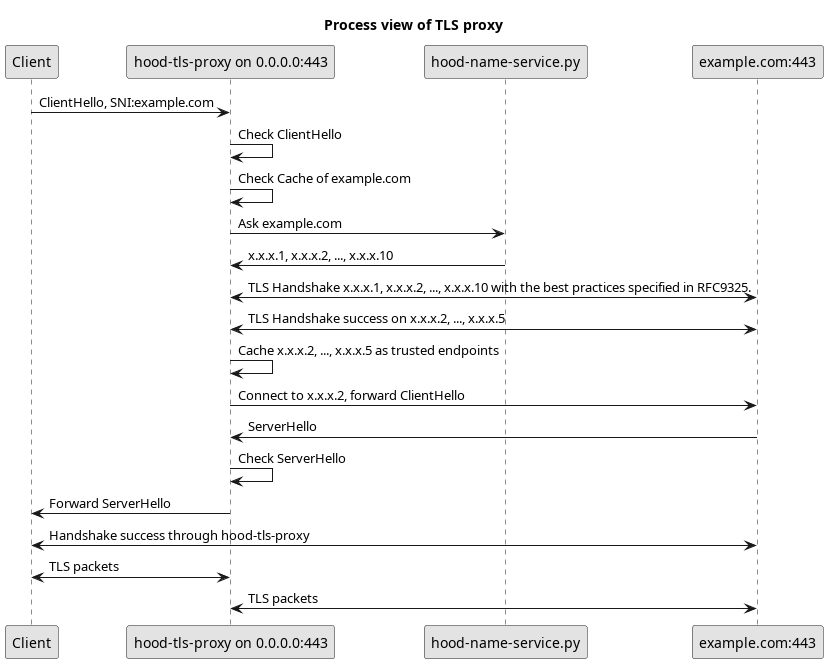
\includegraphics[width=\textwidth]{graphics/puml/process-tls-proxy.png}
  \caption{Process view of TLS proxy}
  \label{fig:tls-proxy-process-view}
\end{figure}

\paragraph{Programming language}
Since TLS proxy is in charge of processing and forwarding the majority of the traffic of the firewall, c++ is used to develop the proxy due to its high-performance capability.
\paragraph{ClientHello}
Upon receiving ClientHello from a client, the proxy first checks the version of the protocol, and the suppor\_versions extension to see if the client supports establishing a safe TLS channel, TLS 1.1 and TLS 1.2 are the only allowed versions \citep{rfc:bstprc}, if a ClientHello shows that the client supports neither, it will be discarded. After the version check, the proxy checks the ciphersuites field, if it contains none of the values listed in \cref{lst:tls-ciphersuites}, it will be considered unable to be safe and discarded \citep{rfc:bstprc}. If a ClientHello passed all of the security checks, the proxy will extract the Server Name Indication (SNI) from the ClientHello to determine the actual destination of the request.

\begin{table}[H]
  \begin{itemize}
    \item TLS\_ECDHE\_RSA\_WITH\_AES\_128\_GCM\_SHA256
    \item TLS\_ECDHE\_RSA\_WITH\_AES\_256\_GCM\_SHA384
    \item TLS\_ECDHE\_ECDSA\_WITH\_AES\_128\_GCM\_SHA256
    \item TLS\_ECDHE\_ECDSA\_WITH\_AES\_256\_GCM\_SHA384
    \item TLS\_AES\_128\_GCM\_SHA256
    \item TLS\_AES\_256\_GCM\_SHA384
    \item TLS\_CHACHA20\_POLY1305\_SHA256
  \end{itemize}
  \caption{Allowed cipher suites values}
  \label{lst:tls-ciphersuites}
\end{table}

\paragraph{Name resolving and trusted endpoint}
The proxy first checks if there are any cached trusted endpoints available, if not it uses a RPC call to hood-name-service.py to resolve the domain name. Then TLS handshakes following the same restrictions to the ClientHello check are made to all of the addresses returned from the name service. The handshake process will not only ensure remote endpoint meets the requirements (versions and ciphersuites) of applying the best practices described in rfc9325, it will also check whether the remote endpoint could provide a valid certificate of the hostname from a trusted CA of the firewall.
\paragraph{ServerHello} After forwarding the ClientHello to the server, a ServerHello will be responded and the proxy will check the final result of the handshake applies to the best practice. If a naughty attacker made the negotiation result unsafe, TLS 1.0 or the cipher suite RSA\_WITH\_NULL\_MD5 for example, the connection will be blocked.

\section{Process view of traffic}
\cref{fig:tls-process-view} shows how a TLS connection interacts with the whole firewall system.
\begin{figure}[H]
  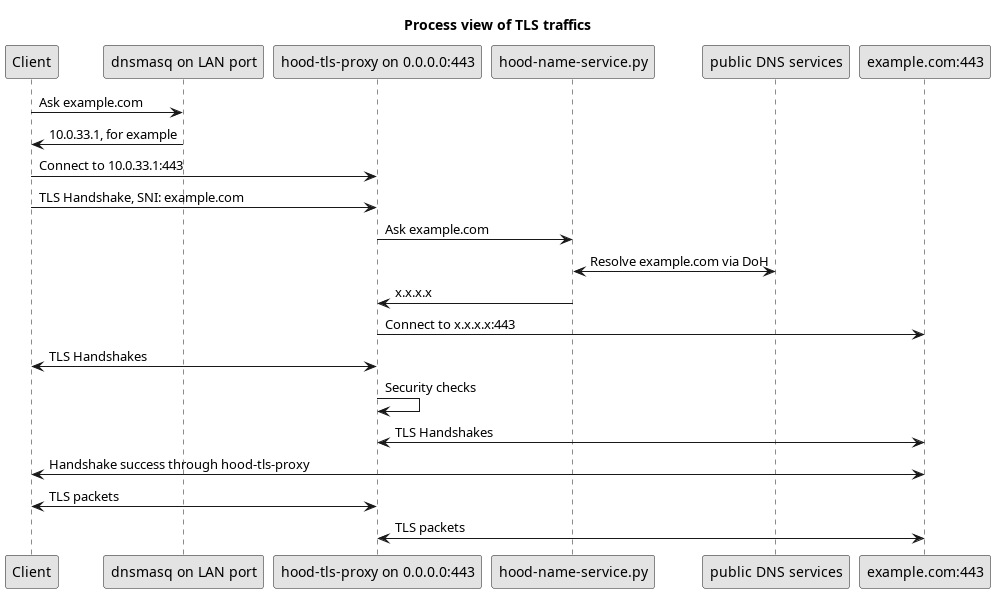
\includegraphics[width=\textheight, angle=90]{graphics/puml/process-tls-traffic.png}
  \caption{Process view of TLS traffic from user}
  \label{fig:tls-process-view}
\end{figure}

\chapter{Plaintext connections}

\section{HTTP}
\subsection{Implementation}
\paragraph{}
hood-http-handler.py is the proxy created to filter and protect HTTP plaintext connections. The proxy checks the host name with a known list of OCSP (Online Certificate Status Protocol) and CRL (Certificate Revocation List) servers. Only the connections to those servers are allowed to be plaintext because those connections usually be OCSP over HTTP connections, which have no reason to be protected. The connections to other servers are tunneled via TLS protocol through the hood-tls-proxy service. See \cref{fig:ocsp-process-view,fig:http-process-view}.

\begin{figure}[H]
  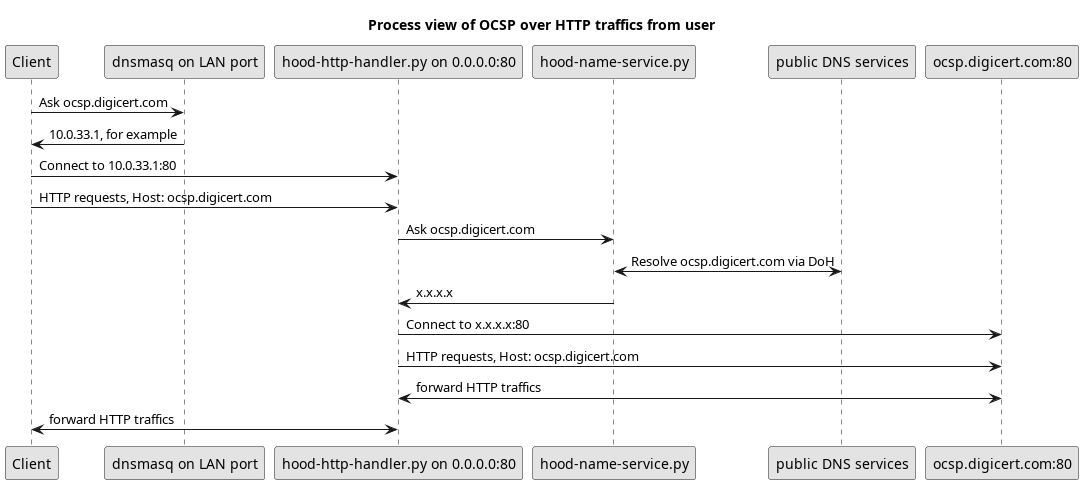
\includegraphics[width=\textheight, angle=90]{graphics/puml/process-ocsp-traffic.png}
  \caption{Process view of OCSP over HTTP traffic from user}
  \label{fig:ocsp-process-view}
\end{figure}

\begin{figure}[H]
  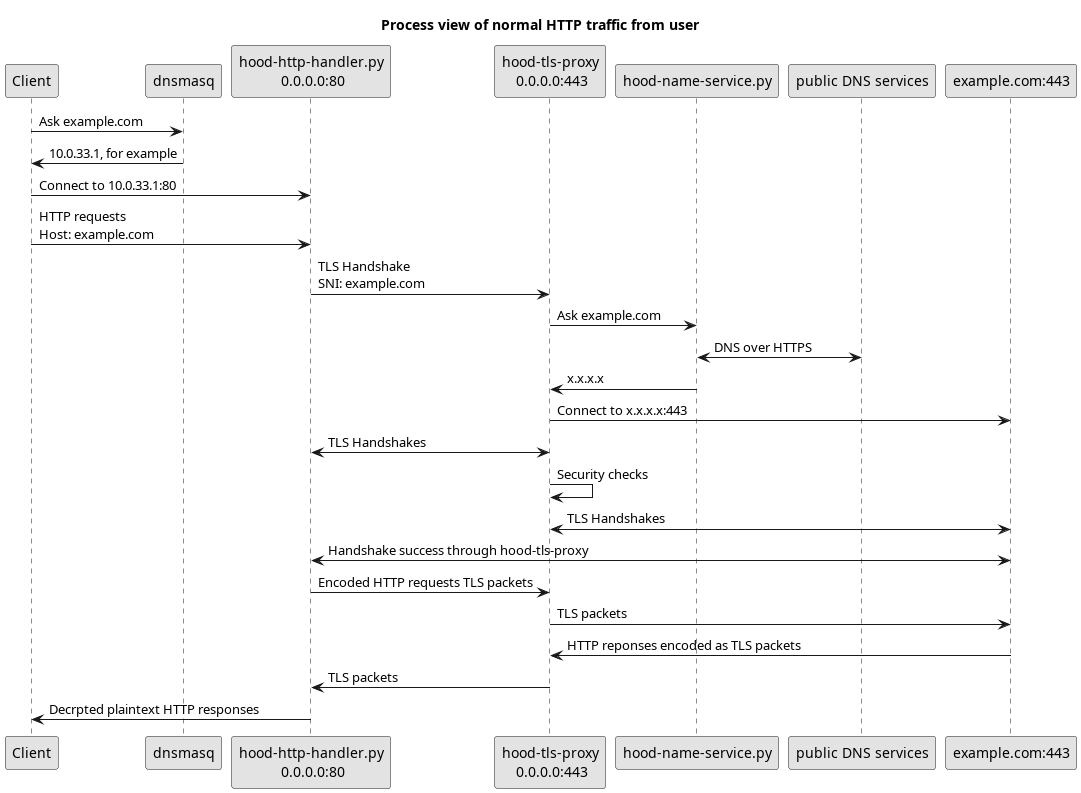
\includegraphics[width=\textheight, angle=90]{graphics/puml/process-http-traffic.png}
  \caption{Process view of normal HTTP traffic from user}
  \label{fig:http-process-view}
\end{figure}

\chapter{Date time synchornization}
\section{Introduction}
\paragraph{}
A correct time is required for TLS protocol to check certificates. Network Time Protocol (NTP) is used by most modern systems to synchronize the clock with a remote server.
\subsection{The issue}
\paragraph{}
A problem with using hardware like a Raspberry Pi is that it does not have a battery to keep the clock ticking after the power source is cut. So a time synchronization mechanism is a must for this firewall.
\paragraph{}
Many operating systems are pre-configured to use an NTP server which has a unique domain name that can be used by a network administrator to identify the operating systems being used by the client.
\paragraph{}
Both the unique port number (UDP 123) and the unique domain names (time.windows.com, time.apple.com, and ubuntu.pool.ntp.org) make NTP a protocol that can be easily identified and targeted. Various attacks can be done to the protocol itself\citep{ntp:attack}. The difference in NTP behavior between different operating systems has been used in OS fingerprinting and tethering detection {osandtether}. Not to mention that the operating system information being exposed by an NTP domain name can also help an attacker target the NTP client being used by the device.

\section{Design}
\paragraph{}
Give up on NTP, use HTTP/HTTPS instead. Use the "Date" header from the response of an HTTP server to synchronize date time with acceptable accuracy. To hide from security detections, the attack vectors targeted to HTTP/HTTPS protocol usually do not want to make mistakes in the header. Even if an attacker targeted the method used by the hood firewall, It's hard to say whether this request is made for time synchronization. Thus the date field of an HTTP response is generally trustworthy.

\section{Implementation}
\paragraph{}
The tool is implemented in a Python script named hood-timesync.py. It accepts two command line arguments as listed in \cref{tab:timesync_cmdarg}. It at first tries to receive an HTTP response through a TLS connection from the domain name specified by the host argument. If it fails, the reason could be the website is down or the system time is too different from the actual time and made a valid certificate unable to pass the validation. Thus, a plaintext connection to the host name provided by the last resort address argument is made as the second attempt. After the second attempt, the tool starts another attempt to receive time from the domain of the host argument via TLS connection, because TLS has less chance to be attacked and because the reason why the first step failed could be the website is temporarily down, the reason could also be the huge time difference made the validation of the certificate failed. In both cases, a HTTPS request to the domain may become possible to succeed after the second attempt. An Epoch time is used as an 'anchor' time. Based on the assumption that time only moves forward, any time before this value will be rejected.

\begin{table}[H]
  \centering
  \begin{tabular}{|c|c|c|m{68mm}|}
    \hline
    Name               & Type & Default      & Description                                                                                                                                                                                                                                               \\
    \hline
    --host             & str  & www.bing.com & The website to request time from                                                                                                                                                                                                                          \\
    --last-resort-host & str  & 1.1.1.1      & The website used as the last resort, should be an IP address                                                                                                                                                                                              \\
    --time-anchor      & int  & 1703703361   & An Epoch time that being anchored as past.\newline Based on the assumption that time only moves forward, any time before this value will be rejected.\newline Set 0 to disable this test.\newline Example: -\-time-anchor=\$(stat /etc/os-release -c \%W) \\
    \hline
  \end{tabular}
  \caption{Command line arguments of hood-timesync.py}
  \label{tab:timesync_cmdarg}
\end{table}

\chapter{Network activity simulation}
\section{Introduction}
\paragraph{}
In this chapter, the goal of the firewall changed to leaking fake information instead of preventing the information leakage because the sad truth is that the combination of all efforts on those protocols is not enough when facing a more sophisticated network analysis. For example, the connections to Windows update servers and App Store servers can be used to detect Windows and Apple devices \citep{osandtether}, but the firewall has no reason to stop those connections. Apart from that, the domain name leaked from TLS handshakes can also tell the eavesdroppers what websites a person is viewing and then may infer what the person is doing. Virtual private networks (VPNs) may prevent that information from being captured by local eavesdroppers but VPNs also have an egress, where could have other eavesdroppers. Thus, when visiting internet websites, the leak of information is inevitable.

\section{Design}
\paragraph{}
A service to simulate different network activities is designed to solve this issue. The goal is to hide user network activities inside the flood of fake network activities to increase the difficulty of an analyzer to produce useful reports. However, the risk of using this service is to produce a false alarm immediately and make the user blocked for tethering, make the user fired for browsing unrelated websites, etc. To prevent the firewall from being compromised by browser vulnerabilities, browser-based simulation tools, like Puppeteer, should not be used for implementation. It should also make plaintext traffic to attract attention from attackers and eavesdroppers to make them less focused on the actual user traffic.

\section{Implementation}
\paragraph{}
The service is implemented in a Python script named hood-actor.py. It can parse and execute action files. To simulate the behaviors of a human user or a computer service. All implementations inside the script are based on the base modules of Python, to avoid the version management of third-party libraries being involved in the installation process of the firewall.

\subsection{Action files}
\paragraph{}
Action files are in JSON format. An action file contains an array of objects. All objects in the array have a "type" field to let the parser know how to process it. Supported object types are descripted in \cref{tab:action_type,tab:properties_object,tab:task_object}.

\begin{table}[H]
  \centering
  \begin{tabular}{|c|c|}
    \hline
    Value      & Description                    \\
    \hline
    properties & Properties of the action       \\
    task       & Tasks to be done in the action \\
    \hline
  \end{tabular}
  \caption{"type" field of action file objects}
  \label{tab:action_type}
\end{table}


\begin{table}[H]
  \centering
  \begin{tabular}{|c|c|c|}
    \hline
    Field       & Type                           & Description                     \\
    \hline
    type        & string                         & "properties"                    \\
    safe\_age   & integer                        & Minimum age safe to do this     \\
    proper\_age & list of two numbers [min, max] & Proper range of age to do this. \\
    \hline
  \end{tabular}
  \caption{"properties" object of action file}
  \label{tab:properties_object}
\end{table}

\begin{table}[H]
  \centering
  \begin{tabular}{|p{34mm}|p{26mm}|p{65mm}|}
    \hline
    Field                   & Type                           & Description                                          \\
    \hline
    type                    & string                         & "task"                                               \\
    name                    & string                         & Name of the task, must be unique in current file     \\
    before                  & list of strings                & Names of tasks that should run no earlier than this. \\
    after                   & list of strings                & Names of tasks that should run before this.          \\
    delay\_between\_actions & list of two numbers [min, max] & Range of seconds to wait between actions.            \\
    actions                 & list of strings                & list hood action script                              \\
    \hline
  \end{tabular}
  \caption{"task" object of action file}
  \label{tab:task_object}
\end{table}

\subsection{HoodExecutor}
HoodExecutor is a general-purpose multi-thread task executor for Python. It can run and schedule in parallel tasks that have dependency relationships and delay requirements. It has a thread pool of workers to execute tasks and a single thread for scheduling delayed tasks. It is required to simulate the paralleled requests sent out from real-world browsers without a third-party HTTP client based on asyncio. It is also the cornerstone of fulfilling all the execution requirements of the tasks and actions in an action file.

\subsection{Browser}\label{sec:browser}
A fake browser is created to simulate network activities of browsing. It records the cookies specified in the HTTP response headers and sends them out like a real browser. It parses the HTML content of the webpage to extract the resources to be loaded and load them in parallel just like a real browser. It uses headers that are used by real browsers and uses different headers on different resources just like a real browser. Cookies are stored in memory and used in the running session. However, due to security concerns, and also to reduce the performance impacts caused by the actor, the fake browser will neither render the webpage [CVE-2023-6707, CVE-2023-6351, CVE-2023-6869, CVE-2023-5170] nor evaluate scripts [CVE-2023-6702, CVE-2023-5997, CVE-2023-5728, CVE-2023-5723] used by the webpage.

\subsection{Hood action script}
\paragraph{}
A hood action script is a script to describe actions to be done to the actor. Each line of the script can be seen as three parts: namespaces, commands, and arguments. For example, \newline "hood:browser:goto:http://www.example.com". "hood:browser:" is to refer browser namespace from the hood namespace, "goto" is a command inside the browser namespace to tell the interpreter to use the browser to load a webpage. "http://www.example.com" is the parameter of the "goto" command. In this example, it represents the URL of the webpage to be loaded.
\subsubsection{hood:browser:goto command}
\paragraph{}
Its usage is "hood:browser:goto URL". Its effect is to use a fake browser (See \cref{sec:browser}) to load a URL. When the special value "random\_link" is used as the argument, the actor randomly picks a link from current webpage of the browser to go to, but nothing will be done if the current webpage contains no links.
\subsubsection{hood:loop command}
\paragraph{}
Its usage is "hood:loop:CONDITION:COMMAND". It is used to declare a loop. Multiple conditions can be declared in the CONDITION part by syntax "key=value[,key=value]". Currently, only two types of conditions are implemented: "exit\_chance" and "delay". "exit\_chance" describes the chance of the loop to be stopped. "exit\_chance=0.33" means the loop has a 33\% chance of termination at the beginning of each loop, "0" means it will never have an end. "1" means the loop will never be executed. "delay" describes the range of delay between each loop. "delay=0-2.5" means the delay between each loop is from 0 seconds to 2.5 seconds. A Just-In-Time compiler is implemented to convert the CONDITION field into Python code. The COMMAND part is the hood action script to be executed in the loop.

\begin{figure}[H]
  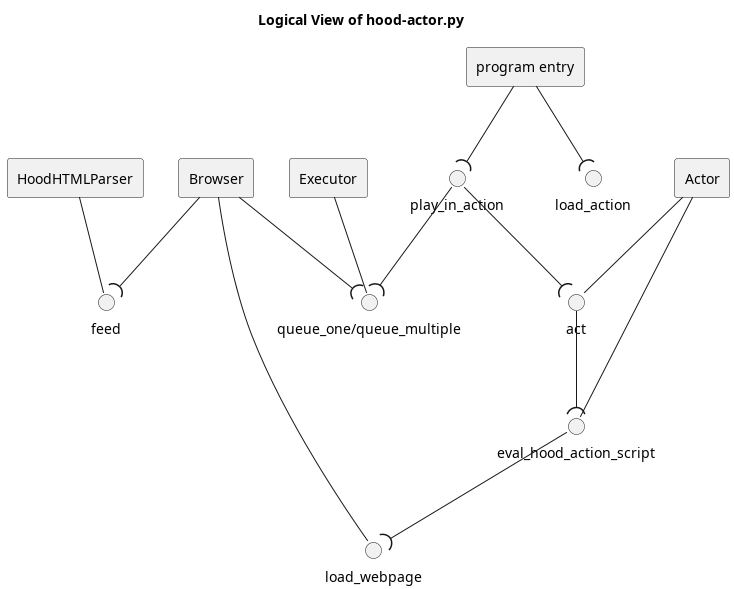
\includegraphics[width=0.9\textwidth]{graphics/puml/actor.png}
  \caption{Logic view of hood-actor.py}
  \label{fig:actor-logic-view}
\end{figure}

\chapter{Dispatcher and firewall rules}\label{cha:dispatcher}
\paragraph{}
Dispatcher is a shell script named 02-hood-dispatcher. It interacts with the changes in the network status or the system status to dynamically configure firewall rules and to start or stop network services. Its callers are three systemctl services: before-network.service (See \cref{sec:before-network-service}), udev.service, and NetworkManager-dispatcher.service.

\section{Initial state of firewall rules}
\paragraph{}
The initial state of firewall rules (See \cref{sec:nftables.conf}) is basic because the design of nftables made the rules with interface name involved requires to be done dynamically. It only allows IPv4 and ARP protocol at layer 3. It allows anything to lo interface but rejects anything else to communicate from 127.0.0.1 or to 127.0.0.1. It allows UDP/TCP packets in connection track established and related
state. It allows the device to send or receive ICMP fragmentation-needed packets. Anything else is ignored.

\section{On udev add event}
\subsubsection{netdev filter}
\paragraph{}
A default netdev filter will be added to both LAN and WAN interfaces. It has to be added dynamically because both its ingress and egress filters require the name of the device. The filter accepts only ARP and IP packets to pass through. The firewall rules from other places already achieved the same thing but it is added because it is the earliest place to filter out a packet and the earlier a packet is filtered the less chance the packet to cause a problem.

\section{On system startup}
\paragraph{}
Upon system startup, the dispatcher will be called by before-network.service. It will start two dmesg instances one is for redirecting firewall-related logs to a log file another is for formatting the log to a more human-readable form. In the iptables era, it was used for initializing iptables rules.
\paragraph{}
Since the udev event could be triggered at a very early stage of the startup, so early that the nftables service may not be available, and adding rules may fail. The dispatcher tries to add a netdev filter on all available network instances again because the timing before-network.service is sufficient to ensure the availability of nftables.service.

\section{On NetworkManager-dispatcher pre-up event}
\paragraph{}
This event means that a network interface is connected to the network but is not yet fully activated. The dispatcher checks the device path with the device specified during the installation process to know whether it is a WAN port. The device path is the real path of the network device. For example, on Linux, the device path of eth0 is the result of "realpath /sys/class/net/eth0".
\subsubsection{WAN port}
\paragraph{}
For the WAN port network interface, the dispatcher allows UDP packets to be sent out from the local 68 port to the remote 67 port and to be received from the remote 67 port to the local 68 port for DHCP protocol.
\subsubsection{LAN port}
\paragraph{}
For LAN port network interfaces, the dispatcher at first picks a randomized start number \(\in [2, 255]\) as the third byte of the IPv4 address, and all following LAN ports use the result of \[2 + (Last Used Number - 1) \mod 254\] as the third byte. The randomization of the start number is made after each system starts. LAN subnet randomization could help increase the difficulty of malicious code in detecting the firewall from the LAN port.
\paragraph{}
After randomization, the following firewall rules are added:
\begin{table}[H]
  \begin{itemize}
    \item Accept the incoming TCP connections through the LAN interface if the destination IP address is the LAN IP address and the destination port is 80 or 443. For hood-http-handler.py and hood-tls-proxy
    \item Accept the incoming UDP packets through the LAN interface if the destination IP address is the LAN IP address and the destination port is 53. For the dnsmasq instance.
    \item Allow UDP packets to be sent out from the local 67 port to the remote 68 port and to be received from the remote 68 port to the local 67 port. For the dnsmasq instance.
  \end{itemize}
  \caption{Firewall rules to be added for LAN ports}
  \label{lst:LAN-rules}
\end{table}
\paragraph{}
A dnsmasq instance is started for this network interface, to assign IP addresses to connected devices, to let connected devices use the IP address of the LAN port of the firewall as the DNS server, and to respond to the IP address of the firewall LAN port for DNS requests.

\section{On NetworkManager-dispatcher up event}
The dispatcher only reacts to this event for the WAN port. It at first waits for DHCP to finish. After DHCP is done, the dispatcher removes DHCP related accept rules from nftables and adds a rule to accept outbound TCP connections from the WAN instance with the source address as the DHCP result to remote 80 and 443 ports. This rule is for HTTP and HTTPS protocols. After that, the dispatcher restarts the hood-network-services.service (\cref{sec:hood-network-services.service}). It will also check the existence of /do\_upgrade or /run\_once files to do a system upgrade or to run the script.

\section{On NetworkManager-dispatcher down event}
The dispatcher removes the firewall rules dynamically added for this instance and kills the dnsmasq instances for this interface.

\chapter{Installation}
\paragraph{}
Installation now can only be done from Linux. install.sh is the shell script that is in charge of the installation process. It copies and applies the scripts, executables, and configuration files to the target Raspberry Pi OS filesystem. It accepts the command line arguments listed in \cref{tab:install_arg}.

\begin{table}[H]
  \centering
  \begin{tabular}{|m{27mm}|m{30mm}|m{68mm}|}
    \hline
    Name                              & Default                                                                         & Description                                                                  \\
    \hline
    usb\_tether=                      & 1                                                                               & Share network to computer via USB cable                                      \\
    harden\_only=                     & 0                                                                               & Only apply hardening parts. Let the target SBC can still used as a computer. \\
    disable\_wireless=                & 1                                                                               & Disable WiFi and Bluetooth.                                                  \\
    disable\_gpu=                     & 1                                                                               & Disable GPU.                                                                 \\
    target=                           & /                                                                               & The target root/device to install firewall.                                  \\
    wan\_port\_\newline device\_path= & /sys/devices/\newline platform/scb/\newline fd580000.ethernet/\newline net/eth0 & The path of the device to be used as WAN port.                               \\
    \hline
  \end{tabular}
  \caption{Command line arguments of install.sh}
  \label{tab:install_arg}
\end{table}

\section{Checking target system}
Multiple checks to the target path are done before the beginning of the installation process to avoid potential harm to the user's computer when they specify a wrong target path. It first checks the type of the target, if the target path is not a directory target will be treated as a device or file and will be mounted as the pattern of a live system of Raspberry Pi OS. If the target is a file, then the target will be mounted as a disk image. If the target does not exist, "/dev/" prefix will be added and will be treated as a name of a device. Then if the content of /boot/firmware/config.txt of the target does not contain the string "dtparam", the target will not be treated as a Raspberry Pi OS filesystem and the installation process will be aborted.

\section{Disable wireless}
Multiple methods are used to ensure the complete disablement of wireless devices. See \cref{tab:config_disable_wireless,tab:delete_disable_wireless}.

\begin{table}[H]
  \centering
  \rowcolors{2}{tablegray}{}
  \begin{tabular}{|m{57mm}|m{68mm}|}
    \hline
    Configuration file                                    & Contents added                                                                                                                                                                                                     \\
    \hline
    boot/firmware/config.txt                              & dtoverlay=disable-bt\newline dtoverlay=disable-wifi                                                                                                                                                                \\
    /etc/modprobe.d/bin-y-disable-wireless-blacklist.conf & blacklist bluetooth\newline blacklist btbcm\newline blacklist hci\_uart\newline blacklist i2c\_brcmstb\newline blacklist i2c\_dev\newline blacklist brcmfmac\newline blacklist brcmutil\newline blacklist cfg80211 \\
    \hline
  \end{tabular}
  \caption{Configurations added to target to disable wireless}
  \label{tab:config_disable_wireless}
\end{table}

\begin{table}[H]
  \begin{itemize}
    \item /lib/firmware/brcm/*
    \item find /lib/linux-image*/broadcom -type f
    \item find /usr/lib/modules/ -name bluetooth
  \end{itemize}
  \caption{Files deleted from target to disable wireless}
  \label{tab:delete_disable_wireless}
\end{table}

\section{Disable GPU}
Multiple methods are used to ensure the complete disablement of GPU. See \cref{tab:config_disable_gpu,tab:delete_disable_gpu}.

\begin{table}[H]
  \centering
  \rowcolors{2}{tablegray}{}
  \begin{tabular}{|m{57mm}|m{68mm}|}
    \hline
    Configuration file                               & Contents modified                                                                                    \\
    \hline
    boot/firmware/config.txt                         & Removed:\newline dtoverlay=vc4-kms-v3d\newline dtoverlay=vc4-fkms-v3d                                \\
    /etc/modprobe.d/bin-y-disable-gpu-blacklist.conf & Added:\newline blacklist v3d\newline blacklist drm\newline blacklist drm\_panel\_orientation\_quirks \\
    \hline
  \end{tabular}
  \caption{Configurations modified to target to disable GPU}
  \label{tab:config_disable_gpu}
\end{table}

\begin{table}[H]
  \begin{itemize}
    \item Any directory under /usr/lib/modules/ with the name "gpu"
  \end{itemize}
  \caption{Files deleted from target to disable GPU}
  \label{tab:delete_disable_gpu}
\end{table}

\begin{landscape}
  \section{Other configurations modified}
  \begin{table}[H]
    \rowcolors{2}{tablegray}{}
    \begin{tabular}{|p{70mm}|p{40mm}|p{80mm}|}
      \hline
      Configuration file                                                                       & Contents modified                                                                                                   & Purpose                                                                            \\
      \hline
      /boot/firmware/cmdline.txt                                                               & Added:\newline ipv6.disable=1\newline apparmor=1\newline security=apparmor                                          & disable IPv6\newline enable AppArmor                                               \\
      /etc/modprobe.d/bin-y-blacklist.conf                                                     & Added:\newline blacklist ipv6\newline blacklist hci\_uart\newline blacklist i2c\_brcmstb\newline blacklist i2c\_dev & disable IPv6, i2c, and UART                                                        \\
      /boot/firmware/config.txt                                                                & Added:\newline enable\_uart=0                                                                                       & disable UART                                                                       \\
      /etc/nftables.conf                                                                       & See \cref{sec:nftables.conf}                                                                                        & nftables rules                                                                     \\
      /etc/hosts                                                                               & OMITTED                                                                                                             & provide address of some DNS services                                               \\
      /etc/sysctl.conf                                                                         & OMITTED                                                                                                             & sysctl related hardening                                                           \\
      /etc/rc.local                                                                            & OMITTED                                                                                                             & host name randomization                                                            \\
      /etc/pki/nssdb/cert9.db\newline /etc/pki/nssdb/key4.db\newline /etc/ca-certificates.conf & OMITTED                                                                                                             & manage trusted certificates                                                        \\
      /etc/NetworkManager/NetworkManager.conf                                                  & OMITTED                                                                                                             & MAC address randomization                                                          \\
      /etc/apt/sources.list\newline /etc/apt/sources.list.d/raspi.list                         & OMITTED                                                                                                             & use HTTPS mirrors for apt                                                          \\
      files related to systemd services                                                        & OMITTED                                                                                                             & enable hood services, enable required system services, and disable unsafe services \\
      \hline
    \end{tabular}
    \caption{Configurations modified to target to disable GPU}
    \label{tab:other_config}
  \end{table}
\end{landscape}


\chapter{Showing network activities}
\paragraph{}
Network activities of the firewall system are logged to multiple places by multiple services (see \cref{tab:network_log}). All logs are simplified to human-readable forms and aggregated to a tty device to let users access them easily. If the firewall was installed with the parameter harden\_only=1, aggregated logs will be sent to tty8, and if the installation parameter harden\_only was 0, aggregated logs will be sent to tty1.
\begin{table}[H]
  \rowcolors{2}{tablegray}{}
  \begin{tabular}{|p{95mm}|p{95mm}|}
    \hline
    Service              & Log location                   \\
    \hline
    hood-name-service.py & /var/log/hood-name-service.log \\
    hood-http-handler.py & /var/log/hood-http-handler.log \\
    hood-tls-proxy       & /var/log/hood-tls-proxy.log    \\
    hood-dispatcher      & /var/log/hood-dispatcher.log   \\
    nftables             & dmesg                          \\
    \hline
  \end{tabular}
  \caption{Log locations of network services.}
  \label{tab:network_log}
\end{table}



\chapter{Analyzation to security events}
\paragraph{}
This chapter analyzes security events and provides reasons why many things that could bring convenience are disabled in the firewall.

\section{Apple security releases}
\begin{figure}[H]
  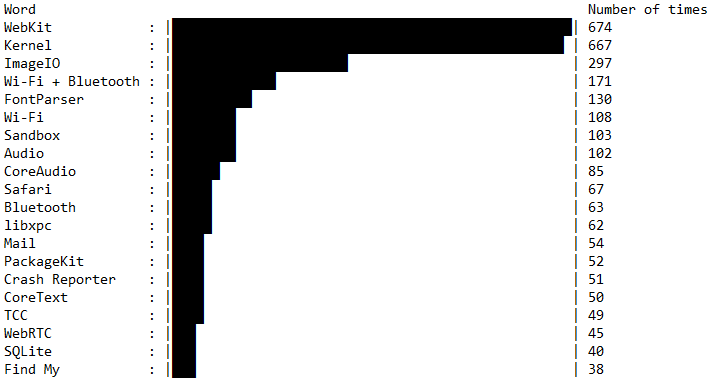
\includegraphics[scale=1]{data/apple_security_releases/result.png}
  \caption{Top 15 mostly mentioned components in Apple security releases\newline from Januray 8th 2020 to Januray 12th 2024}
  \label{fig:apple-sec-release}
\end{figure}
\paragraph{}
I collected texts of Apple security releases of its operating systems between Januray 8th 2020 and Januray 12th 2024 from Apple website and then counted the number of times of an component being mentioned in their security releases. See \cref{fig:apple-sec-release}. They are the top 15 mostly mentioned components with one exception: the number of "Wi-Fi + Bluetooth" is the sum of the two.
\paragraph{}
The result explains how risky using a browser could be: WebKit, the underlying engine of Safari is the top 1 on the list, the browser Safari itself is the 9th place, and many things related to browsing are on the list: ImageIO, FontParser, CoreText, and WebRTC. Without the time spent on creating a 'fake' browser, the simulation of web-browsing network activity may have to choose between crude bash scripts or dangerous browser-based tools.
\paragraph{}
It also demonstrates why firewall disables wireless by default: Both "Wi-Fi" and "Bluetooth" are on the list, and their sum can take the fourth place.

\section{IPv6}
\paragraph{}
This section explains why firewall disables IPv6 by default. I searched both the keyword "IPv6" and the keyword "IPv4" from the website \url{https://cve.mitre.org}. On Jan 14th 2024 (UTC +1) 00:00, there are 615 CVE records that match the keyword "IPv6" and 360 CVE records that match the keyword "IPv4". From 2022, there are 81 results match the keyword "IPv6" and 36 result match the keyword "IPv4". Those numbers indicate that the overall implementations of IPv6 is less stable than of IPv4. It could be explained as IPv4 implementations have a longer history of bug fixes.

\section{GPU}
One of the reasons to disable GPU is a stealthy GPU-based keylogger reported on EUROSEC 2013. TODO:ref

\chapter{Conclusions}
As conclusion, the decisions on disabling things are supported by numbers and related threats.

\section{Possible improvements for future}
\subsection{LSM and seccomp}
\paragraph{}
Use LSMs, like AppArmor, and seccomp to protect as many processes as possible. The programs that do not support seccomp can be changed by LD\_LOAD\_LIBRARY.

\subsection{Compile time hardening}
\paragraph{}
Use strict compiler options to harden everything, including kernel, like what Gentoo Linux is doing now, to try to mitigate some unpublished vulnerabilities, and also to increase the difficulty of attacking the firewall itself.

\subsection{Network stack fingerprinting}
\paragraph{}
Spoof network stacks, like TCP stacks and TLS stacks, make the firewall and the devices behind it to be less detectable.

\subsection{Further use to libcomposite}
\paragraph{}
Libcomposite can make the device show multiple roles to a host (a computer), which means the device can at the same time work as a USB mass storage device or as a USB CDROM, both of which can be used as a media of a Live DVD. Then the computer will be able to boot a live system from it. For a computer that is password protected to boot from USB, we can also use this small device as a PXE server to make that computer boot from the network of the USB device.

\appendix 

\chapter{Simple scripts and services created by firewall}

\section{before-network.service}\label{sec:before-network-service}
before-network.service is a systemd service being enabled during installation process and run before network is available to system. It is created to trigger dispatcher (See \cref{cha:dispatcher}) to initialize firewall rules and network configurations.

\section{hood-network-services.service}\label{sec:hood-network-services.service}
It is a service for running hood network services. It runs hood-network-services-runner.sh which starts hood-http-handler.py, hood-name-service.py, hood-tls-proxy, and a dnsmasq client for DNS queries made from the firewall system.

\section{allowd\_tls\_ports.txt}\label{sec:allowed_tls_ports.txt}
TLS is widely applied to secure protocols, not just for HTTP. This file is created to support more TLS-encrypted protocols in the future. It is a text file with lines of port numbers. Lines starting with \# are treated as comments and are ignored. Ports listed in the file will be allowed in nftables rules by the dispatcher and will be handled by hood-tls-proxy.

\section{domain\_blacklist.txt}\label{sec:domain_blacklist.txt}
It is a text file with lines of regular expressions. Lines starting with \# are treated as comments and are ignored. Domains matching any one of the regular expressions in the file will be blocked.

\section{ip\_subnet\_blacklist.txt}\label{sec:ip_subnet_blacklist.txt}
It is a text file with lines of IP subnets. Lines starting with \# are treated as comments and are ignored. IP addresses matching any one of the subnets in the file will be blocked.

\section{nftables.conf}\label{sec:nftables.conf}
\begin{lstlisting}{language=conf}
#!/usr/sbin/nft -f

flush ruleset

table ip filter {
  chain input {
    type filter hook input priority filter; policy drop;
    iif lo accept
    ip daddr 127.0.0.1/8 log prefix "[HOOD D]" flags all drop 
    ip saddr 127.0.0.1/8 log prefix "[HOOD D]" flags all drop
    meta l4proto udp ct state {established, related} log prefix "[HOOD A]" flags all accept
    ct state {established, related} accept
    icmp type {destination-unreachable} icmp code {frag-needed} accept
    log prefix "[HOOD D]" flags all drop
  }
  chain forward {
    type filter hook forward priority filter; policy drop;
    log prefix "[HOOD D]" flags all drop
  }
  chain output {
    type filter hook output priority filter; policy drop;
    oif lo accept
    ip daddr 127.0.0.1/8 log prefix "[HOOD D]" flags all drop 
    ip saddr 127.0.0.1/8 log prefix "[HOOD D]" flags all drop 
    meta l4proto udp ct state {established, related} log prefix "[HOOD A]" flags all accept
    ct state {established, related} accept
    icmp type destination-unreachable icmp code {frag-needed} accept
    log prefix "[HOOD D]" flags all drop
  }
}

table ip6 filter {
  chain ingress {
    type filter hook input priority filter; policy drop;
    log prefix "[HOOD D]" flags all drop
  }
  chain prerouting {
    type filter hook input priority filter; policy drop;
    log prefix "[HOOD D]" flags all drop
  }
  chain input {
    type filter hook output priority filter; policy drop;
    log prefix "[HOOD D]" flags all drop
  }
  chain forward {
    type filter hook forward priority filter; policy drop;
    log prefix "[HOOD D]" flags all drop
  }
  chain output {
    type filter hook output priority filter; policy drop;
    log prefix "[HOOD D]" flags all drop
  }
  chain postrouting {
    type filter hook forward priority filter; policy drop;
    log prefix "[HOOD D]" flags all drop
  }
}

table bridge filter {
  chain ingress {
    type filter hook input priority filter; policy drop;
    log prefix "[HOOD D]" flags all drop
  }
  chain prerouting {
    type filter hook prerouting priority filter; policy drop;
    log prefix "[HOOD D]" flags all drop
  }
  chain input {
    type filter hook output priority filter; policy drop;
    log prefix "[HOOD D]" flags all drop
  }
  chain forward {
    type filter hook forward priority filter; policy drop;
    log prefix "[HOOD D]" flags all drop
  }
  chain output {
    type filter hook output priority filter; policy drop;
    log prefix "[HOOD D]" flags all drop
  }
  chain postrouting {
    type filter hook postrouting priority filter; policy drop;
    log prefix "[HOOD D]" flags all drop
  }
}

table netdev filter {
}


table arp filter {
  chain input {
    type filter hook input priority filter; policy drop;
  }
  chain output {
    type filter hook output priority filter; policy drop;
  }
}
\end{lstlisting}

\chapter{The attacks encountered during the time I was working on this thesis}

\section{Malicious hardwares}
\paragraph{}
Normal attackers will use the network, Bluetooth, or WiFi for communications between malware and the host. For example, casting the screen to another device via WiFi or sending keyboard inputs via Bluetooth. Those kinds of attacks can be detected by an RF detector. RF shielding fabric, RF detectors, and signal jammers could be used to fight against such kinds of attacks.
\paragraph{}
However, there are still other methods. Some even without wireless communications. Despite I had already bought an RF detector to alert me of wireless communications between unknown hardware, unknown attackers still managed to monitor my progress with some modified hardware. Take the devices that I am using to develop this project for example. Raspberry 4B has a USB chip that can communicate with the power source. If the charger is specially crafted with the ability to forward the USB connection to the remote endpoint via power lines, then, with the help of the malware installed on the Pi itself, data can be leaked silently via power lines even without any network connections to the computer. The same story can also happen to the portable screen that I am using now. I have found two counter measurements to this kind of attack: One is to use a USB-C to DC adapter when connecting a USB-C charger to the laptop. Another is to tape the two pins in the middle of the male USB-A port to prevent data communications.

\section{Sounds}

\paragraph{}
Another attack that can bypass a computer without a wireless device, is to use AI / ML to identify the sounds of keyboard hits. The detected types can be sent to remote via power lines or mobile phones. The sound could even be recorded from the room of a neighbor which makes this attack more stealthy than other methods. I use cardboards to extend the pillar of the key cap to shorten the key travel to lower the volume of the sound of the key hit to counter this attack but I am uncertain about the effect because I have no attack tools to test this. AliPay also used to use sound waves to transmit data between phones and vending machines. My Raspberry Pi recently started to emit strange noises from the speakers on the screen, which could be because of the same kind of technology being used by hackers.


\backmatter

\chapter{Glossary} %optional
\section{CDC-ECM}\label{sec:CDC-ECM}
\paragraph{}
It is the Ethernet Control Model (ECM) Devices subclass of Universal Serial Bus (USB) Communication Device Class (CDC). It's specification is available on the website \url{http://www.usb.org}. It provides a virtual ethernet link to host OS but it is not supported by most of Apple products.

\section{RNDIS}\label{sec:RNDIS}
\paragraph{}
The Remote Network Driver Interface Specification (RNDIS) is a Microsoft proprietary protocol. It provides a virtual ethernet link to host OS but it is not supported by Microsoft Windows.

\section{nftables}\label{sec:nftables}
\paragraph{}
Nftables is the modern Linux kernel packet classification framework. It is available in Linux kernels >= 3.13.
%\bibliographystyle{alpha}
%\bibliographystyle{dcu}
\bibliographystyle{plainnat}
\bibliography{biblio}

%\cleardoublepage
%\theindex %optional, use only if you have an index, must use
%\makeindex in the preamble
%\lipsum
1
\end{document}
\grid
